\begin{figure}[h]
    \centering
    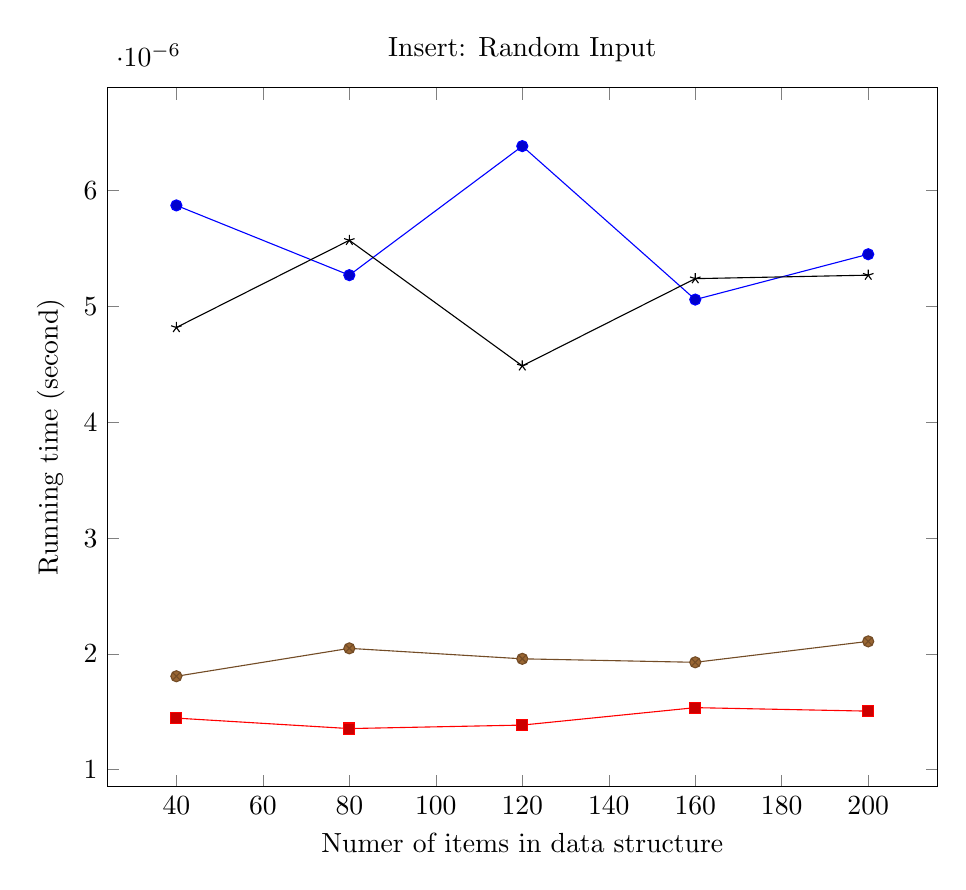
\begin{tikzpicture}
        \begin{axis}[
            xlabel={Numer of items in data structure},
            ylabel={Running time (second)},
            title={Insert: Random Input},
            width=\textwidth
        ]
		\addplot coordinates {
			(40, 5.872919066657323e-06)
			(80, 5.270568393153652e-06)
			(120, 6.384917139136415e-06)
			(160, 5.059745657427783e-06)
			(200, 5.451273595205586e-06)
		};
		\addplot coordinates {
			(40, 1.4456416164085328e-06)
			(80, 1.3552890153825659e-06)
			(120, 1.3854065490578882e-06)
			(160, 1.535994217433112e-06)
			(200, 1.5058766837577896e-06)
		};
		\addplot coordinates {
			(40, 1.807052020511013e-06)
			(80, 2.0479922899108162e-06)
			(120, 1.9576396888848492e-06)
			(160, 1.927522155209527e-06)
			(200, 2.108227357261461e-06)
		};
		\addplot coordinates {
			(40, 4.818805388026593e-06)
			(80, 5.571743729906875e-06)
			(120, 4.487512517598047e-06)
			(160, 5.2404508594783294e-06)
			(200, 5.270568393153652e-06)
		};
        \legend{}
        \end{axis}
    \end{tikzpicture}
    \caption{Average of 0 operations, benchmarked every 0, starting at 0.}
\end{figure}